\documentclass[a4paper,10pt]{article}
\usepackage[utf8]{inputenc}
\usepackage{times}
\usepackage[margin=2cm]{geometry}
\usepackage{booktabs}
\usepackage{graphicx}
\usepackage{enumitem}
\usepackage{tikz}
\usetikzlibrary{arrows.meta}
\setlist{itemsep=1pt,topsep=3pt}
\newcommand{\opt}[1]{\texttt{-{}-#1}}

% Lab record: at most two pages. Keep the section structure.

\title{Fault-Tolerant Distributed Systems -- Lab record}
\author{Lab \textbf{1} -- Group \textbf{G}: member 1, member 2, member 3, member 4}
\date{}

\begin{document}

\maketitle
\vspace{-3em}

\section*{1. Claim}

\noindent\emph{Under assumptions} 3 servers, crash-stop failures, messages
delayed, reordered or lost by partitions (never duplicated or corrupted),
asynchronous timing, \emph{if at most} $f=2$ servers \emph{other than n0}
\emph{fail by} crashing or being partitioned from n0, \emph{the service
guarantees} linearizable \texttt{read}/\texttt{write}/\texttt{cas}, and
answers to the clients of n0 and of every server still connected to n0.
Linearizability holds for \emph{any} number of failures, n0 included; but
with n0 down no client is answered, and in a partition the clients of
servers cut off from n0 are not answered.\\
\emph{Evidence:} 19 Maelstrom \texttt{lin-kv} runs of \texttt{d.py}, all
valid (table below), including 3 partition runs and 3 runs with n0 crashed;
plus the structural argument: one authoritative copy, executed one
operation at a time, the only one ever read.\\
\emph{Not covered:} any availability when n0 is down (no failover:
0~crashes of n0 tolerated); n0 restarting without memory; duplicated
messages; durability (backups' copies can be stale and divergent).

\section*{2. Design and predictions}

\textbf{Strategy D, primary for everything.} A backup (n1, n2) forwards
every client request unchanged to n0 and relays n0's reply to the client;
no timeout, no local answers. n0 executes the request on its copy; after a
successful \texttt{write}/\texttt{cas} it sends \texttt{update\{key,
value\}} (the new value) to the backups, fire and forget, then replies.
Backups overwrite their copy on \texttt{update}; nobody reads it. No acks,
sequence numbers, retries or failover (not part of D).

\begin{center}
\footnotesize
\begin{tabular}{@{}llll@{}}
\toprule
Scenario & Predicted & Observed: \emph{all valid}; ok/fail/info & Why it differs \\
\midrule
No faults & valid; all complete & 150/59/0, 160/50/0, 125/74/0 & -- \\
\opt{latency 50} \opt{rate 50} & valid; slower & 744/270/0, 698/270/0, 711/295/0 & median 108\,ms at backups, 8\,ms \\
 & & & at n0: only 2 delayed hops, not 4\\
\texttt{MS\_CRASH=n0@5} & valid; none after 5\,s & 0 ok after 5\,s; 45/45/44 info & -- \\
\texttt{MS\_CRASH=n1@5} & valid; n1's clients stop & n1's clients: 0 ok after 5\,s; 9/6/8 info & -- \\
\opt{nemesis partition} & valid; cut-off side stops & 124/55/8, 117/72/10, 143/53/4 & -- \\
\midrule
\opt{latency 100} \opt{rate 100} & valid & 1039/361/0, 1017/378/0, 1026/356/0 & extra: try to break it \\
\texttt{MS\_CRASH=n0@5-12} & valid; resumes at 12\,s & 95/55/21 (1 run); 43 ok after 13\,s & extra: n0 paused \\
\bottomrule
\end{tabular}
\end{center}
\vspace{-0.5em}
\noindent (\emph{fail} includes cas mismatches, missing keys, and reads that
timed out: Maelstrom records a timed-out read as \emph{fail}, not
\emph{info}.)

\section*{3. Evidence}

Run \texttt{runs/p4-partition} (= \texttt{store/lin-kv/20261016T180341.995+0100};
partition, valid, 124/55/8). At 11.144\,s the nemesis isolates n0 from n1 and n2 until the
end. From then on, n0's clients complete 49 operations, n1's and n2's
none: 0 forwarded requests reach n0 and 0 updates reach the backups (last
\texttt{apply}: 10.484\,s, $x=4$).

\begin{center}
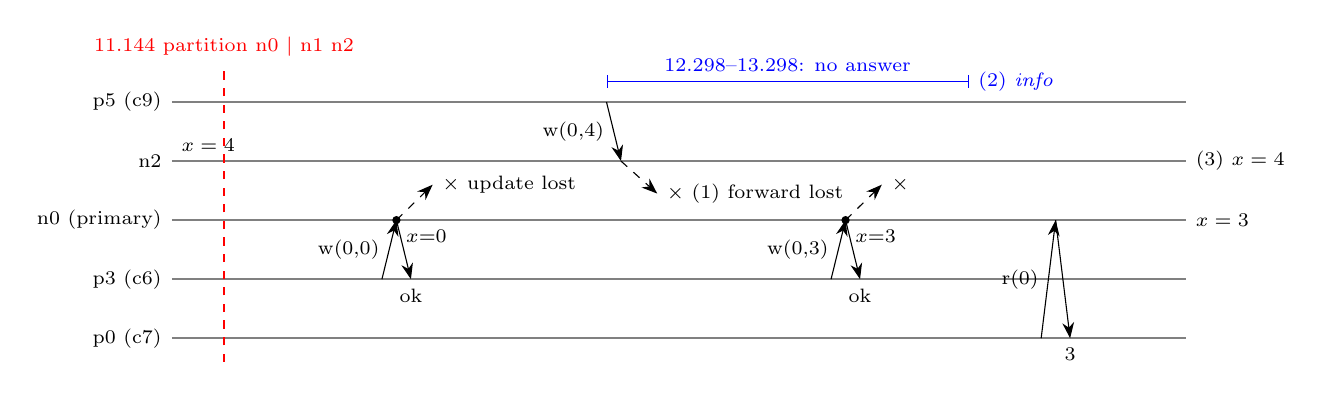
\begin{tikzpicture}[x=0.92cm,y=0.75cm,>={Stealth[length=2mm]},font=\scriptsize]
  \foreach \y/\l in {4/{p5 (c9)},3/{n2},2/{n0 (primary)},1/{p3 (c6)},0/{p0 (c7)}}
    \draw[thick,gray] (0,\y) node[left,black]{\l} -- (14,\y);
  % partition
  \draw[red,dashed,thick] (0.72,-0.4) -- (0.72,4.6) node[above]{11.144 partition n0 $|$ n1 n2};
  \node[above right] at (0,3) {$x=4$};
  % p3 write(0,0) at n0
  \draw[->] (2.9,1) -- node[left]{w(0,0)} (3.1,2);
  \fill (3.1,2) circle (1.5pt) node[below right]{$x{=}0$};
  \draw[->] (3.1,2) -- (3.3,1) node[below]{ok};
  \draw[->,dashed] (3.1,2) -- (3.6,2.6) node[right]{$\times$ update lost};
  % p5 write(0,4) via n2
  \draw[->] (6.0,4) -- node[left]{w(0,4)} (6.2,3);
  \draw[->,dashed] (6.2,3) -- (6.7,2.45) node[right]{$\times$ (1) forward lost};
  \draw[|-|,blue] (6.0,4.35) -- node[above]{12.298--13.298: no answer} (11.0,4.35);
  \node[blue,right] at (11.0,4.35) {(2) \emph{info}};
  % p3 write(0,3)
  \draw[->] (9.1,1) -- node[left]{w(0,3)} (9.3,2);
  \fill (9.3,2) circle (1.5pt) node[below right]{$x{=}3$};
  \draw[->] (9.3,2) -- (9.5,1) node[below]{ok};
  \draw[->,dashed] (9.3,2) -- (9.8,2.6) node[right]{$\times$};
  % p0 read
  \draw[->] (12.0,0) -- node[left]{r(0)} (12.2,2);
  \draw[->] (12.2,2) -- (12.4,0) node[below]{3};
  % end state
  \node[right] at (14,3) {(3) $x=4$};
  \node[right] at (14,2) {$x=3$};
\end{tikzpicture}
\end{center}
\vspace{-0.5em}
(1)~The forwarded \texttt{write(0,4)} is dropped by the partition; under D,
n2 may not answer by itself. (2)~p5 records \emph{info}: the traces show
the write was never executed, but p5 cannot tell this from ``executed, reply
lost''; the checker may leave it out, which is consistent with p0 reading 3.
(3)~The copies diverge (n2: 4, n0: 3), invisibly, since nobody reads n2.
This does not violate our specification (linearizability, as the checker):
every \emph{ok} result comes from n0's one copy in n0's execution order. It
does violate availability for 2/3 of the clients.

\section*{4. Limitations and open questions}

\begin{itemize}
\item Valid runs are not a proof; our confidence rests on the argument
  that faults can only remove answers. 20\,s runs, 3 nodes, few keys.
\item No failover: as soon as a backup answers or takes over, the
  divergence of (3) becomes a stale read, and n0 may still be alive (split
  brain). Next: let n1 take over after a timeout, and observe the anomaly.
\item Not injectable with \texttt{ms.py}: n0 restarting \emph{without} its
  memory, duplicated messages. Next: longer partitions, more nodes,
  longer runs.
\item Open: how to make a backup a safe successor --- acks from (a
  majority of) backups before replying, ordered updates, agreement on who
  is primary.
\end{itemize}

\section*{5. AI log}

\begin{itemize}
\item Claude Code was asked to ``complete the lab for strategy D'' (an
  \emph{answer directly} request, against the guide's
  think-first workflow: noted here). It restated D and the open details
  first; the group checked them against its own design.
\item It wrote \texttt{kv.py}, \texttt{d.py} and scripts to run each
  scenario 3 times and record verdict/counts; it kept to D (no acks,
  timeouts or failover) as \texttt{AGENTS.md} requires.\item Corrected/learnt from the runs, not from the assistant's prediction:
  timed-out reads are \emph{fail}, not \emph{info}; \opt{latency}
  delays only server-to-server messages; a backup timeout must not answer
  error 11 (n0 may have executed the request).
\item \emph{(Group: add what you accepted, changed or rejected.)}
\end{itemize}

\section*{6. Contributions}

\begin{itemize}
\item member 1: \dots
\item member 2: \dots
\item member 3: \dots
\item member 4: \dots
\end{itemize}

\end{document}
